\documentclass{standalone}
\usepackage{tikz}
\usetikzlibrary{positioning}
\begin{document}
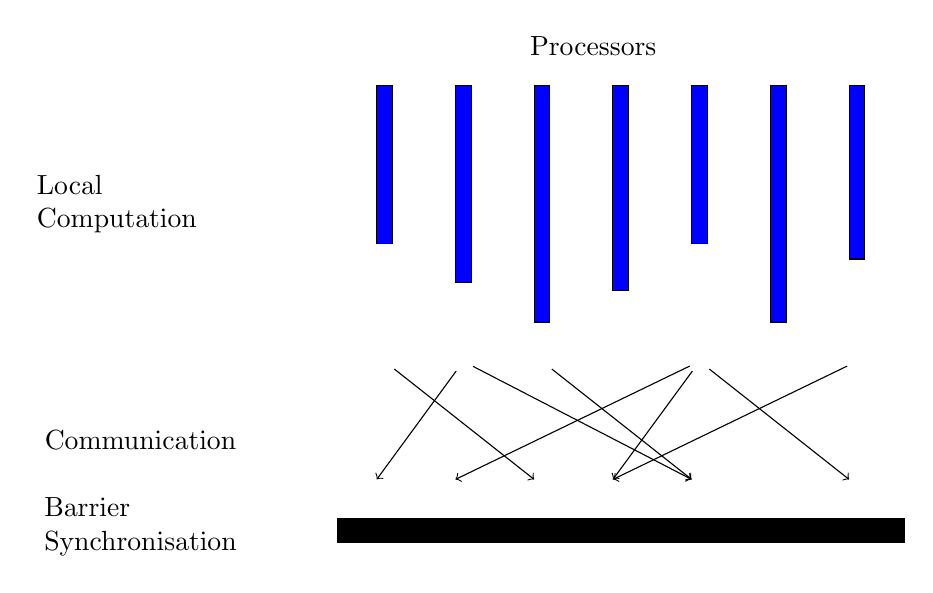
\begin{tikzpicture}
    \foreach \h [count=\i] in {2,2.5,3,2.6,2,3,2.2}
        {
            % local computation
            \draw[fill=blue] (\i,0) rectangle (\i+.2,-\h);
            %arrow start
            \node (A\i) at (\i+.1,-3.5) {};
        }
    % communication
    \draw[->] (A1) -- (3,-5);
    \draw[->] (A2) -- (1,-5); \draw[->] (A2) -- (5,-5);
    \draw[->] (A3) -- (5,-5);
    \draw[->] (A5) -- (2,-5); \draw[->] (A5) -- (4,-5); \draw[->] (A5) -- (7,-5);
    \draw[->] (A7) -- (4,-5);
    % barrier
    \draw[fill=black] (.5,-5.5) rectangle (7.7,-5.8);
    % text label
    \node (p) at (3.75,.5) {Processors};
    \node[align=left] (p) at (-2.3,-1.5) {Local\\ Computation};
    \node[align=left] (p) at (-2,-4.5) {Communication};
    \node[align=left] (p) at (-2,-5.6) {Barrier\\Synchronisation};
\end{tikzpicture}
\end{document}